\chapter{Related Works}
\label{ch:relatedworks}

機器翻譯是利用電腦自動模擬產生人們文本翻譯的結果,本研究將目前的機器翻譯系統分成三大類:Rule-based machine translation, Example-based machine translation及Statistical machine translation分別敘述如下:


Rule-based machine translation:這類方法是將翻譯的規則以條列式的方式列出,翻譯的過程中遇到何種情況,則依照規則採取不同的行動。


Example-based machine translation:這類方法則是利用訓練語料中有出現過最符合的句子當作樣本來進行翻譯,因此如果是出現在訓練語料中的句子,此種方法相較於其他方法正確性更高。


Statistical machine translation:這類方法則是利用訓練語料,訓練出不同的翻譯模型,之後利用這些翻譯模型來對翻譯原始句進行翻譯。


以上三種不同的方式,各自有其優點及缺點,因此才會有機器翻譯整合系統的延伸,希望能夠合併各種不同系統的優點,來補足單一系統的不足,而在\cite{ayan2008iab}中,將機器翻譯整合系統分成三個不同的層級分別是:Sentence level combination, Phrase level combination 及Word level combination,以下將依照這三種不同的分類,進行深入的探討。

\section{Sentence level combination}
\label{sec:slc}
Sentence level combination,是利用各種不同的特徵函數,利用Minimum Error Rate Training\cite{och2003mer}來取得各個特徵之間的權重,並以此評估各個翻譯假說之好壞,輸出最佳者當作其翻譯結果\cite{hildebrand:cmt},這樣子的系統好處是不需要各個翻譯系統提供任何資料,所有的特徵函數都是利用整合系統自身訓練出來的模型來當作一致的評分標準。而這類系統的特性為所產生的句子,並沒有經過重組,因此必定與其中一個翻譯系統的句子相同。
\begin{figure}[tbh]
  \centering
  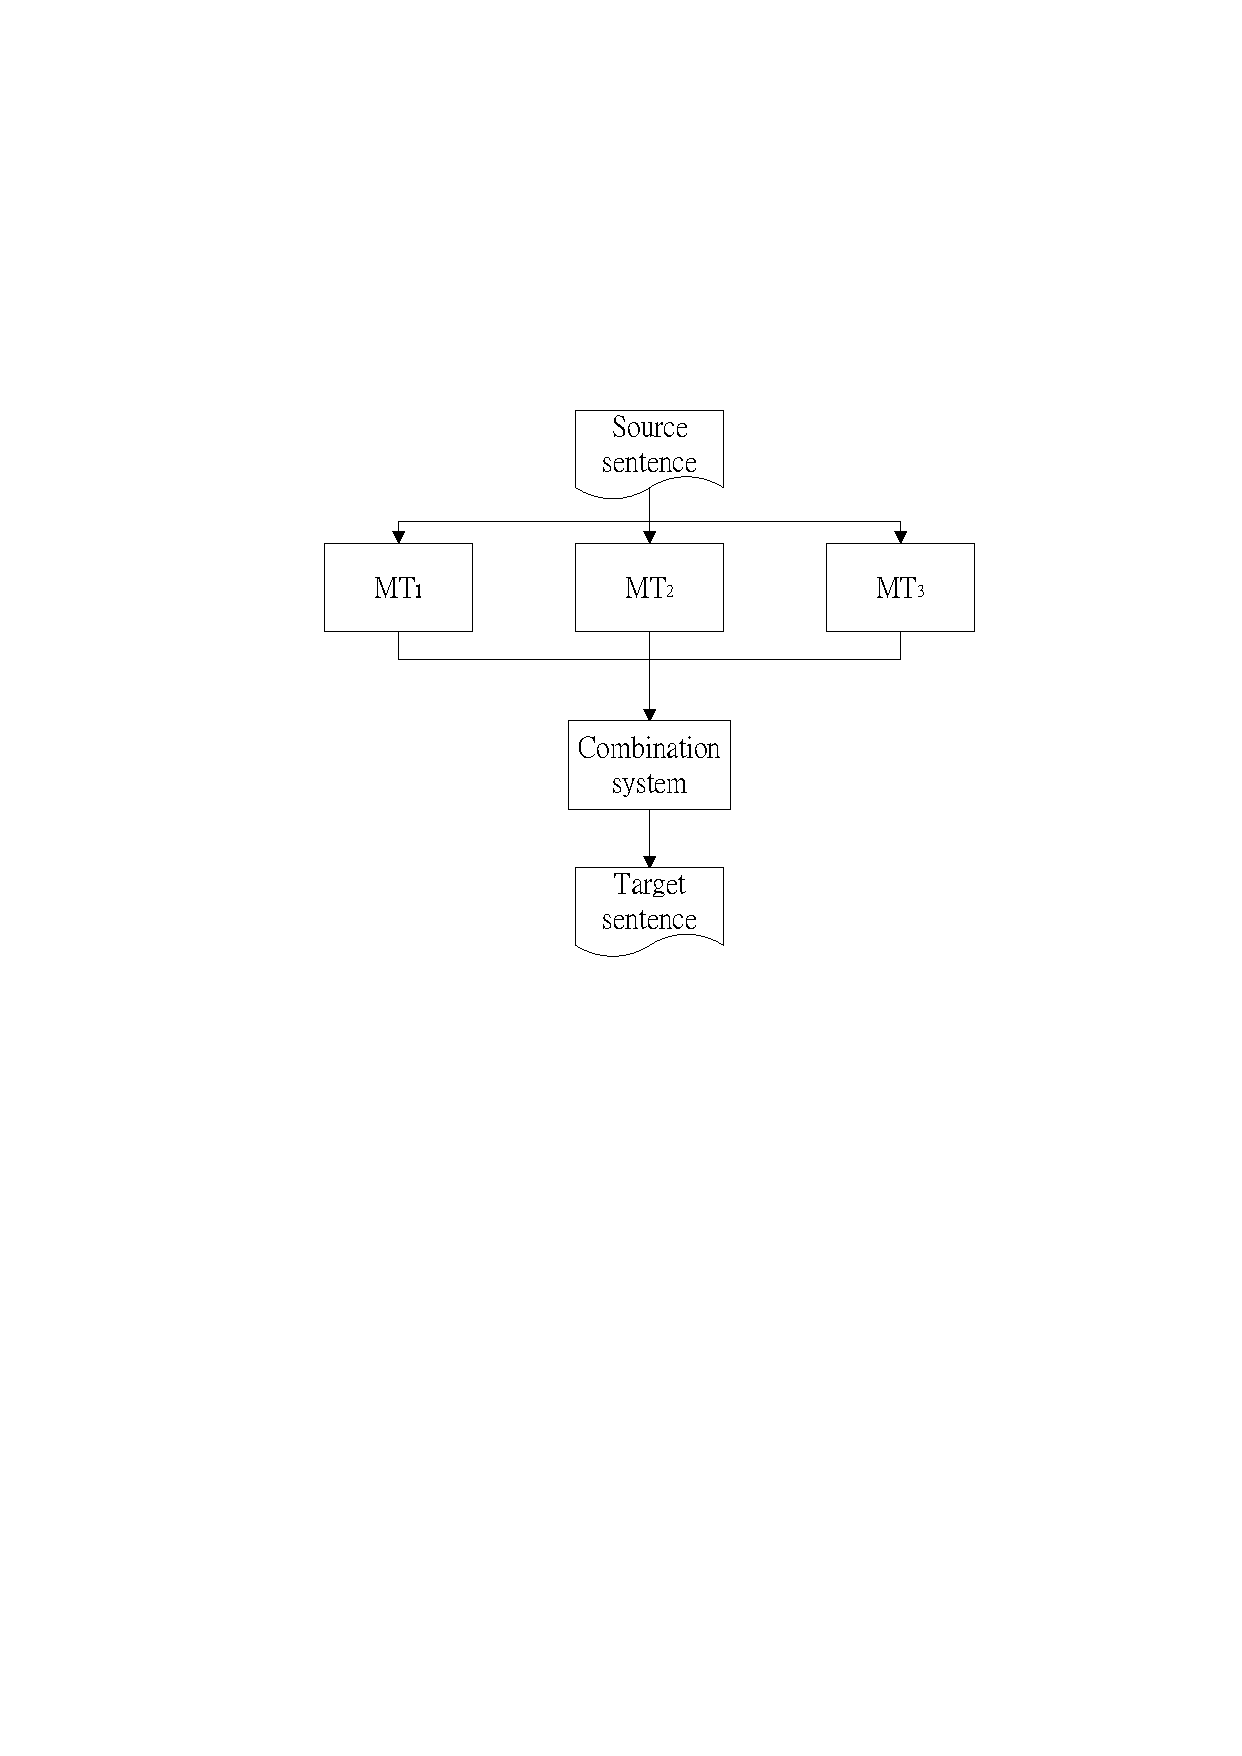
\includegraphics{figs/sentence.pdf}
  \newcommand{\xc}{Sentence level combination 架構}
   \caption[\xc]{\xc.~\textcolor{magenta}}%%{Well, you are right. It looks
    %%  more like a placeholder than a figure showing the proposed
      %%algorithm.}}
  \label{fig:sencom}
\end{figure}
\section{Phrase level combination}
\label{sec:plc}

Phrase level combination,則是取得各個翻譯系統的片語對,如果無法由各個系統取得片語對,則利用GIZA++\cite{och03:asc}對翻譯假說及翻譯原始句進行對齊來取得片語對,之後再利用整合過的片語表來重新進行翻譯\cite{huang2007hsc},此類方法可以解決訓練語料中,片語對不足的問題。而且其翻譯結果並不一定會與先前的翻譯系統類似,因此有機會會輸出比任何一個翻譯系統都還要良好的結果。
\begin{figure}[tbh]
  \centering
  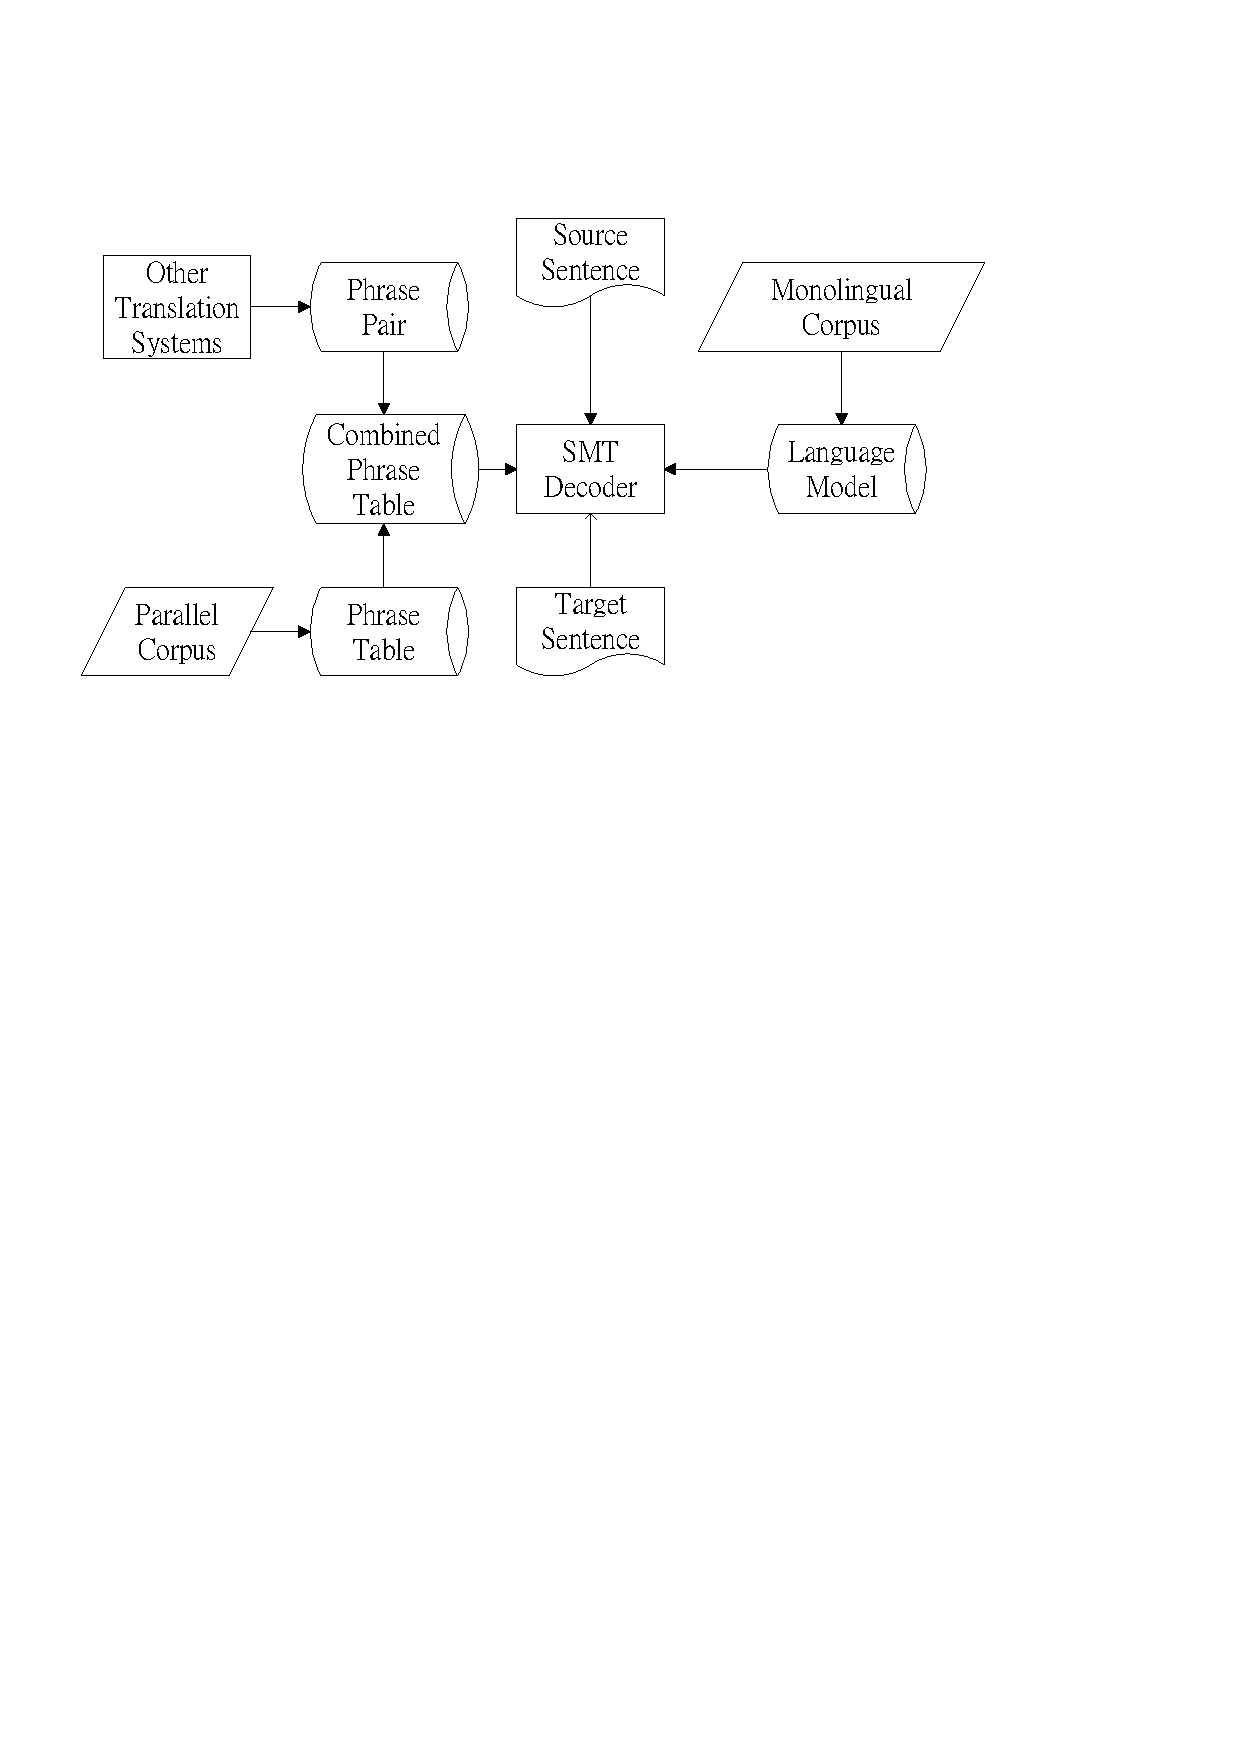
\includegraphics{figs/phrase.pdf}
  \newcommand{\xc}{Phrase level combination 架構}
   \caption[\xc]{\xc.~\textcolor{magenta}}%%{Well, you are right. It looks
    %%  more like a placeholder than a figure showing the proposed
      %%algorithm.}}
  \label{fig:phrasecom}
\end{figure}
\section{Word level combination}
\label{sec:Wlc}

Word level combination方面,主要是將所有的假說,建立成一個confusion network,之後在對這個confusion network計算出最佳的假說,而其一開始的應用並不是被利用於機器翻譯的系統整合上面,而是應用在語音辨識系統整合\cite{fiscus1997pps},而此方法應用在機器翻譯的整合系統上時,相較於語音辨識的整合系統,所需要克服的困難點就是字的排列順序,由於語音辨識系統所輸出的假說只會有一種順序,而機器翻譯系統所輸出的假說所輸出的順序可能有極大的不同,因此我們必須先選擇一個翻譯假說當作對齊的標準,之後將其他翻譯假說對齊到這個標準,並建構出一個confusion network,再由這confusion network選擇出最佳的翻譯假說\cite{bangalore2001cct}。


而在\cite{ayan2008iab}中,更進一步的以confusion network所得到的翻譯假說當作skelton重新進行alignment,得以進一步提昇正確率。


另外在\cite{jayaraman2005mem}的研究,採用了另一種Word level的合併方式,這個方法利用了句子中各個字的詞幹資訊以及part-of-speech(POS)的資訊來進行對齊,而這個方法定義了其最佳對齊是兩個句子之間具有最少的交叉邊,並以此建構成一個word lattice,而系統最後搜尋這個lattice,根據language model以及其他的評分標準產生了最佳的翻譯假說。



%%而在\cite{huang2007hsc},則是依照資料來源的取得將機器翻譯系統整合分成二個不同的類型:Glass-box combinaiton及Black Box combination。

%%\subsection{Glass-box combination}
%%\label{sec:gc}

%%在Glass-box combination,各個不同的機器翻譯系統除了需要提供翻譯假說之外,還必須提供其他額外的資訊,像是翻譯原始句及翻譯目標句的alignemnt以及其他零零總總的資訊,以利整合系統所使用,


%%\section{Information Extraction and Retrieval}
%%\label{sec:irie}


%%\subsection{Information Extraction}
%%\label{sec:ie}


%%\subsection{Information Retrieval}
%%\label{sec:ir}


%%\section{Data and Document Clustering}
%%\label{sec:clustering}


%%\subsection{Data clustering}
%%\label{sec:dataclustering}


%%\subsection{Document Clustering}
%%\label{sec:docclustering}



\section{Discussions}
\label{sec:discussions}

以上幾種不同層級的合成方法,根據\cite{rosti2007com}研究嘗試了三種不同層級的結合方法,發現了採用Word level combination的方法能夠得到較佳的結果,這是因為Word level combination其對於翻譯假說的修正較其他層級的整合系統較廣,因此能夠取得相對較高的改進。
%%Finally, discussions\footnote{\textcolor{magenta}{And probably a footnote in still another color.}} $\ldots$
